	\begin{frame}
	\frametitle{День 9. 26 августа}
	\framesubtitle{\textbf{пер. Кичкинекол Малый (1А, 3206)}~--- д.р. Чунгур-Джар} % Optional subtitle
	\begin{columns}[c] % The "c" option specifies centered vertical alignment while the "t" option is used for top vertical alignment
		\begin{column}{0.55\textwidth} % Left column width
			\begin{itemize}
				\item «Самый лайтовый перевал»
				\item Поляна Крокусов
				\item Гроза
				\item Прошли \textbf{4.6} км
				\item ЧХВ: 2:42
				\item Набор/сброс: \textcolor{darkred}{\textbf{+360}}/\textcolor{darkblue}{\textbf{-520}}~м
			\end{itemize}
			
		\end{column}
		\begin{column}{0.45\textwidth} % Right column width
			\centering
			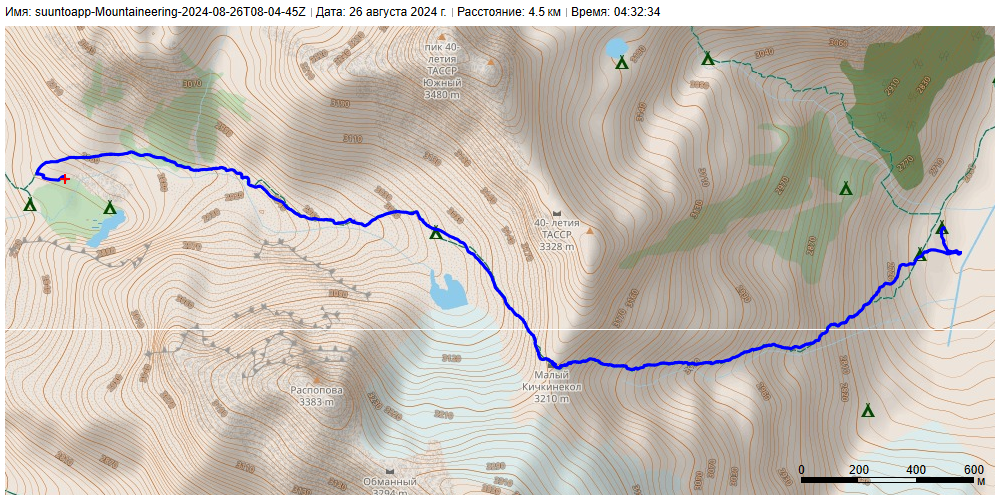
\includegraphics[width=\linewidth]{../pics/mini_maps/26}
		\end{column}
	\end{columns}
\end{frame}

\begin{frame}
	\frametitle{Утро}
	\framesubtitle{День 9, 26 августа}
	\centering
	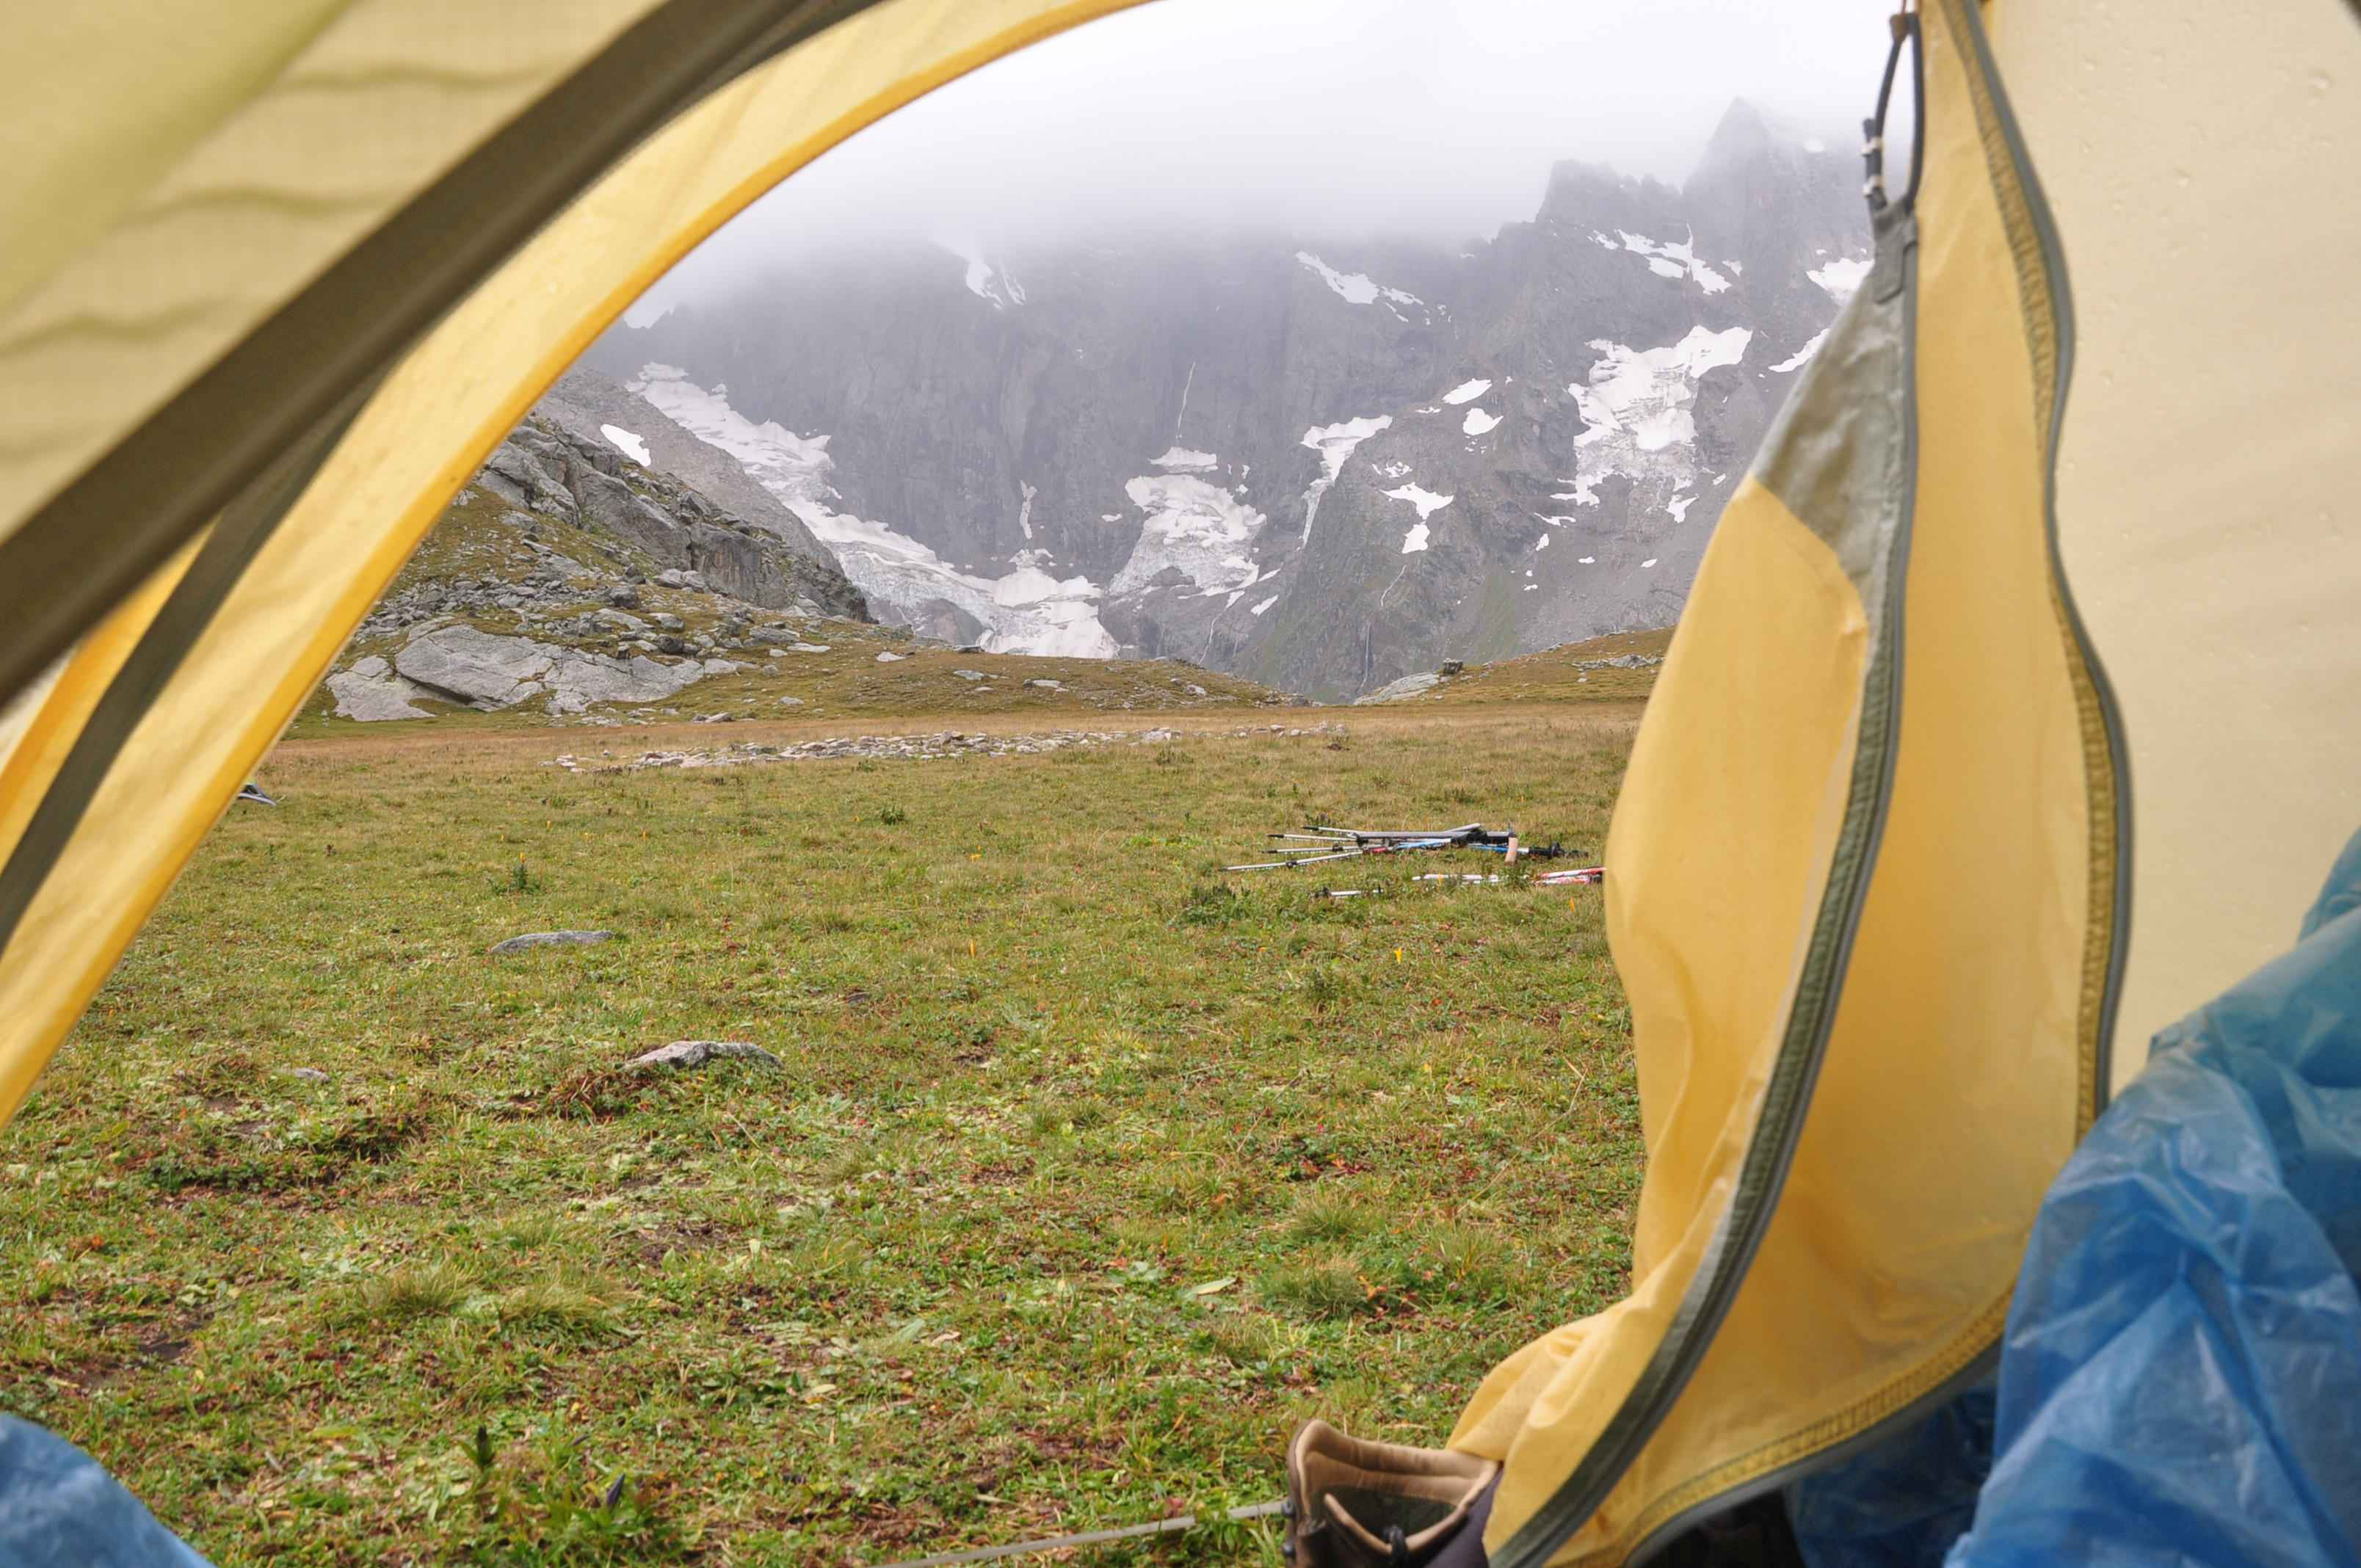
\includegraphics[width=\textwidth]{../pics/DSC_0190}			
\end{frame}

\begin{frame}
	\frametitle{Круг камней}
	\framesubtitle{День 9, 26 августа}
	\centering
	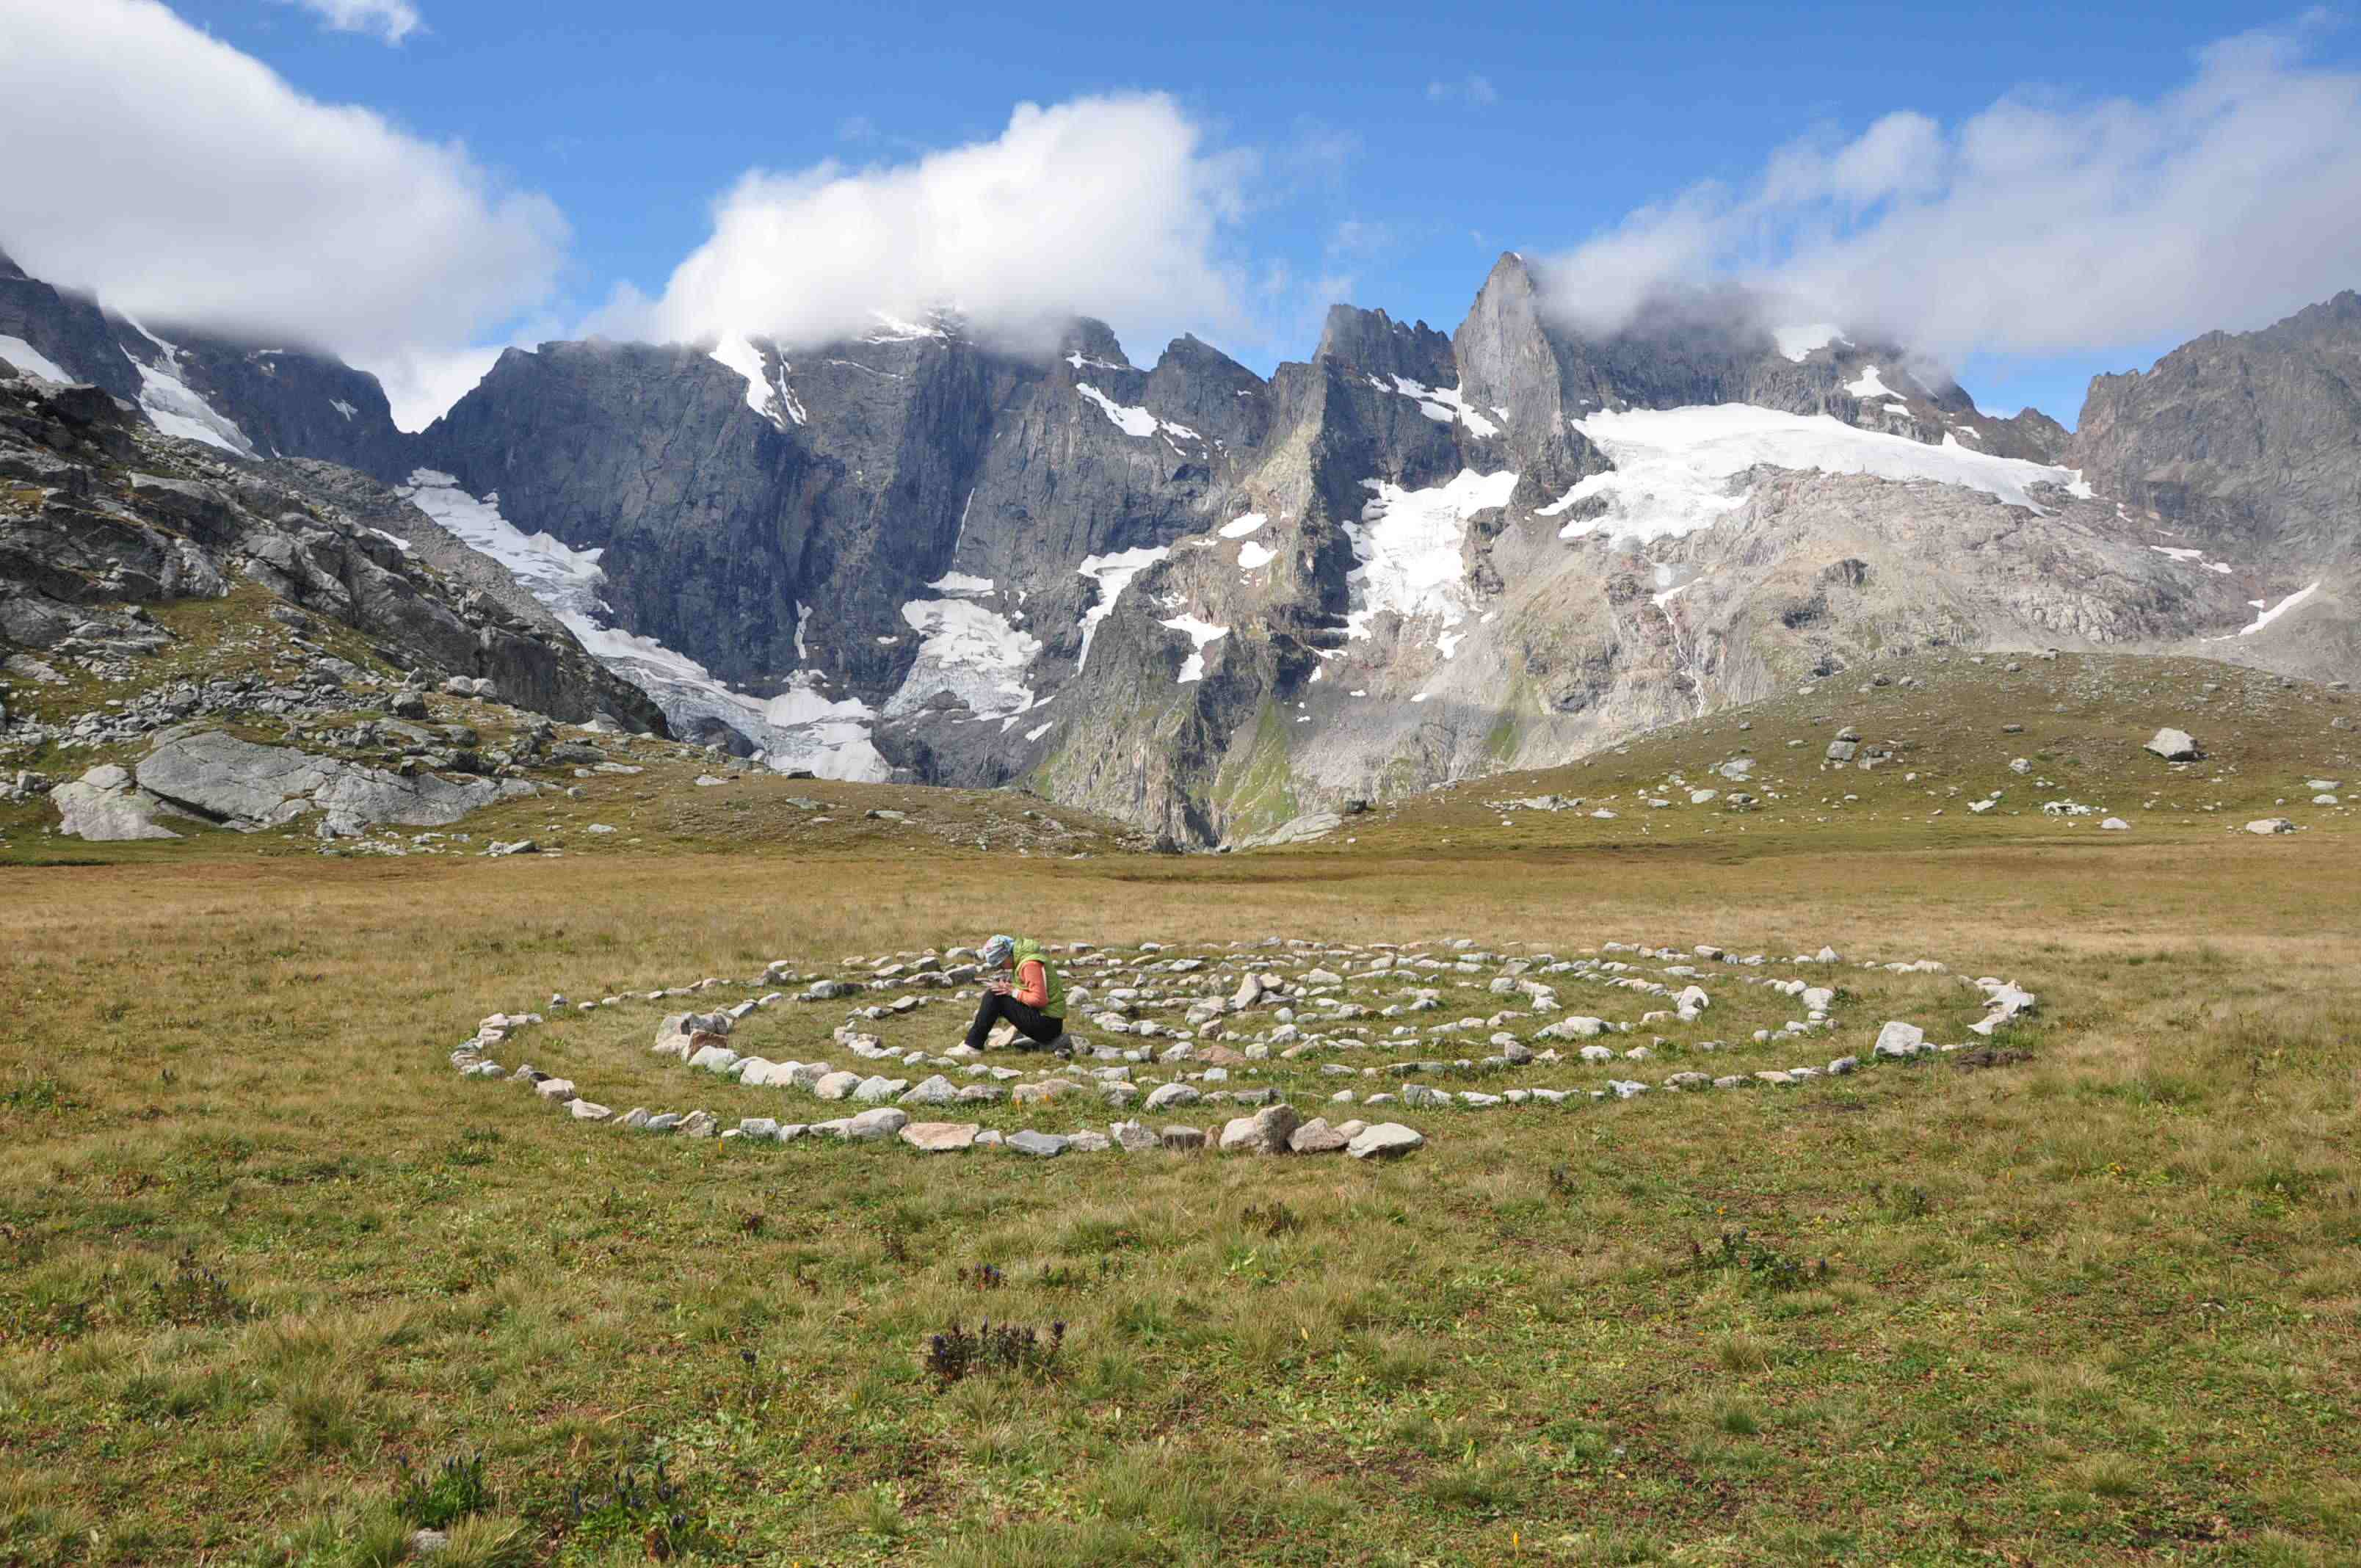
\includegraphics[width=\textwidth]{../pics/DSC_0192}			
\end{frame}

\begin{frame}
	\frametitle{Козлы}
	\framesubtitle{День 9, 26 августа}
	\centering
	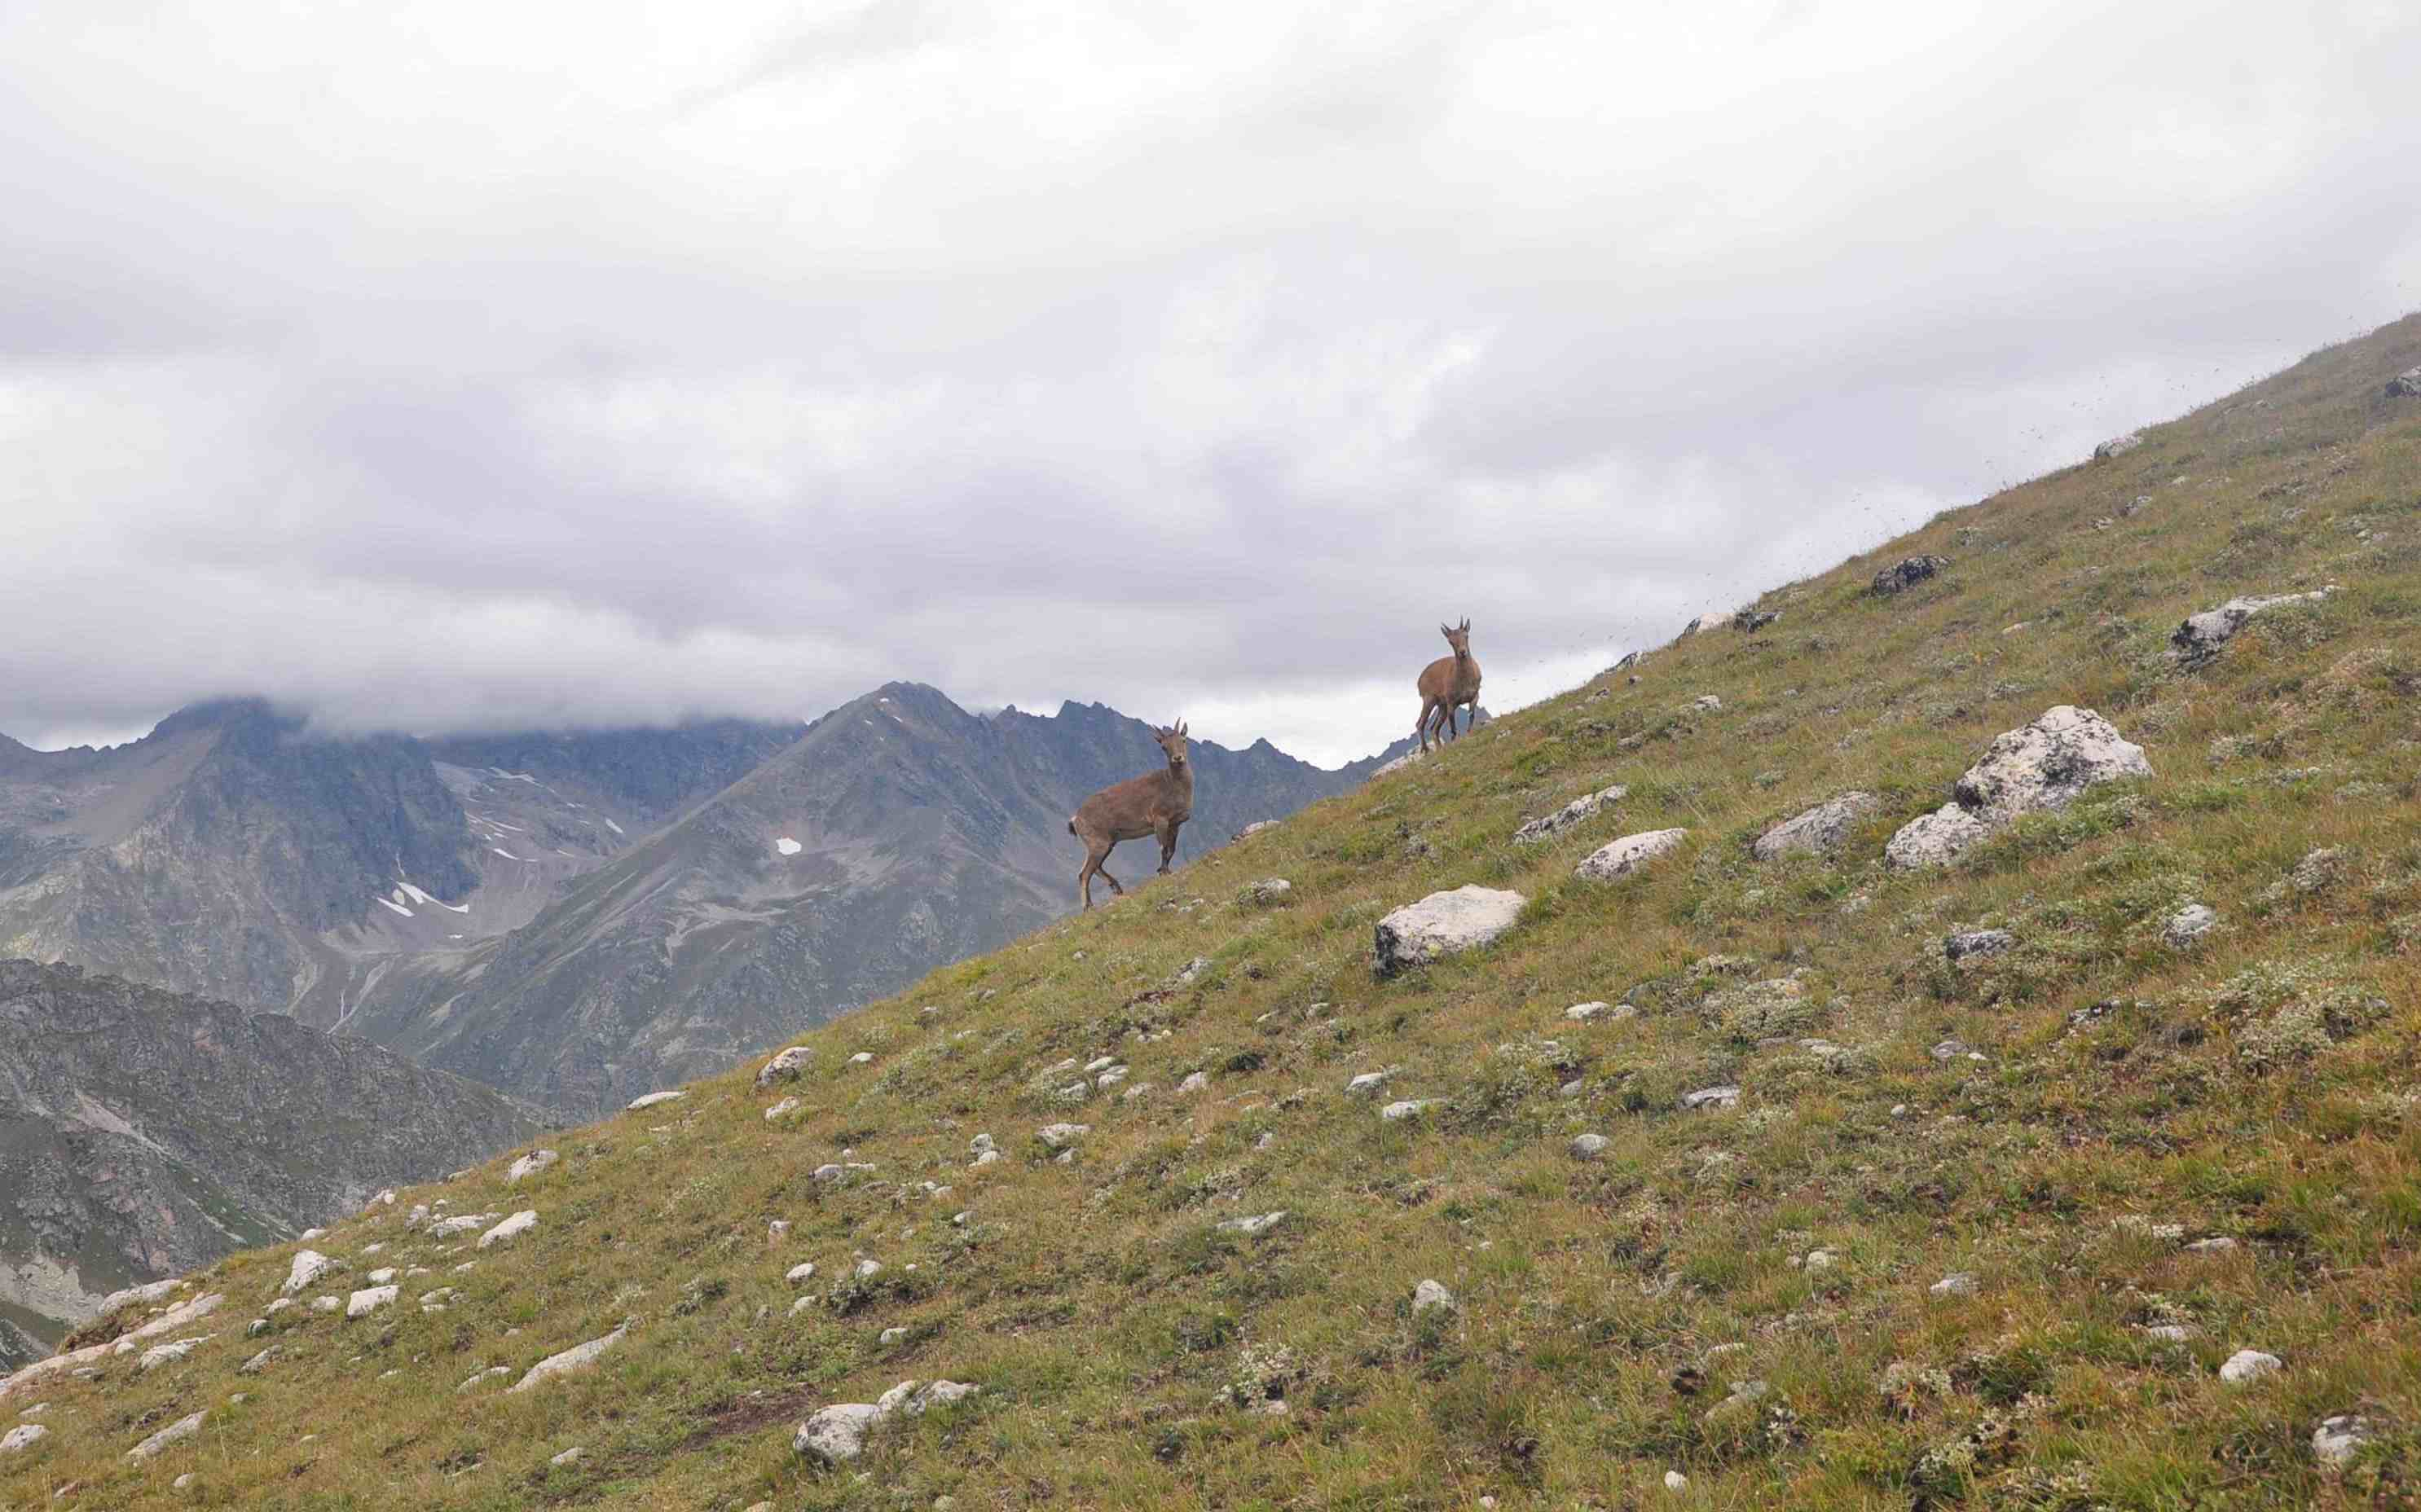
\includegraphics[width=\textwidth]{../pics/DSC_0211}			
\end{frame}

\begin{frame}
	\frametitle{Атмосфера дня}
	\framesubtitle{День 9, 26 августа}
	\centering
	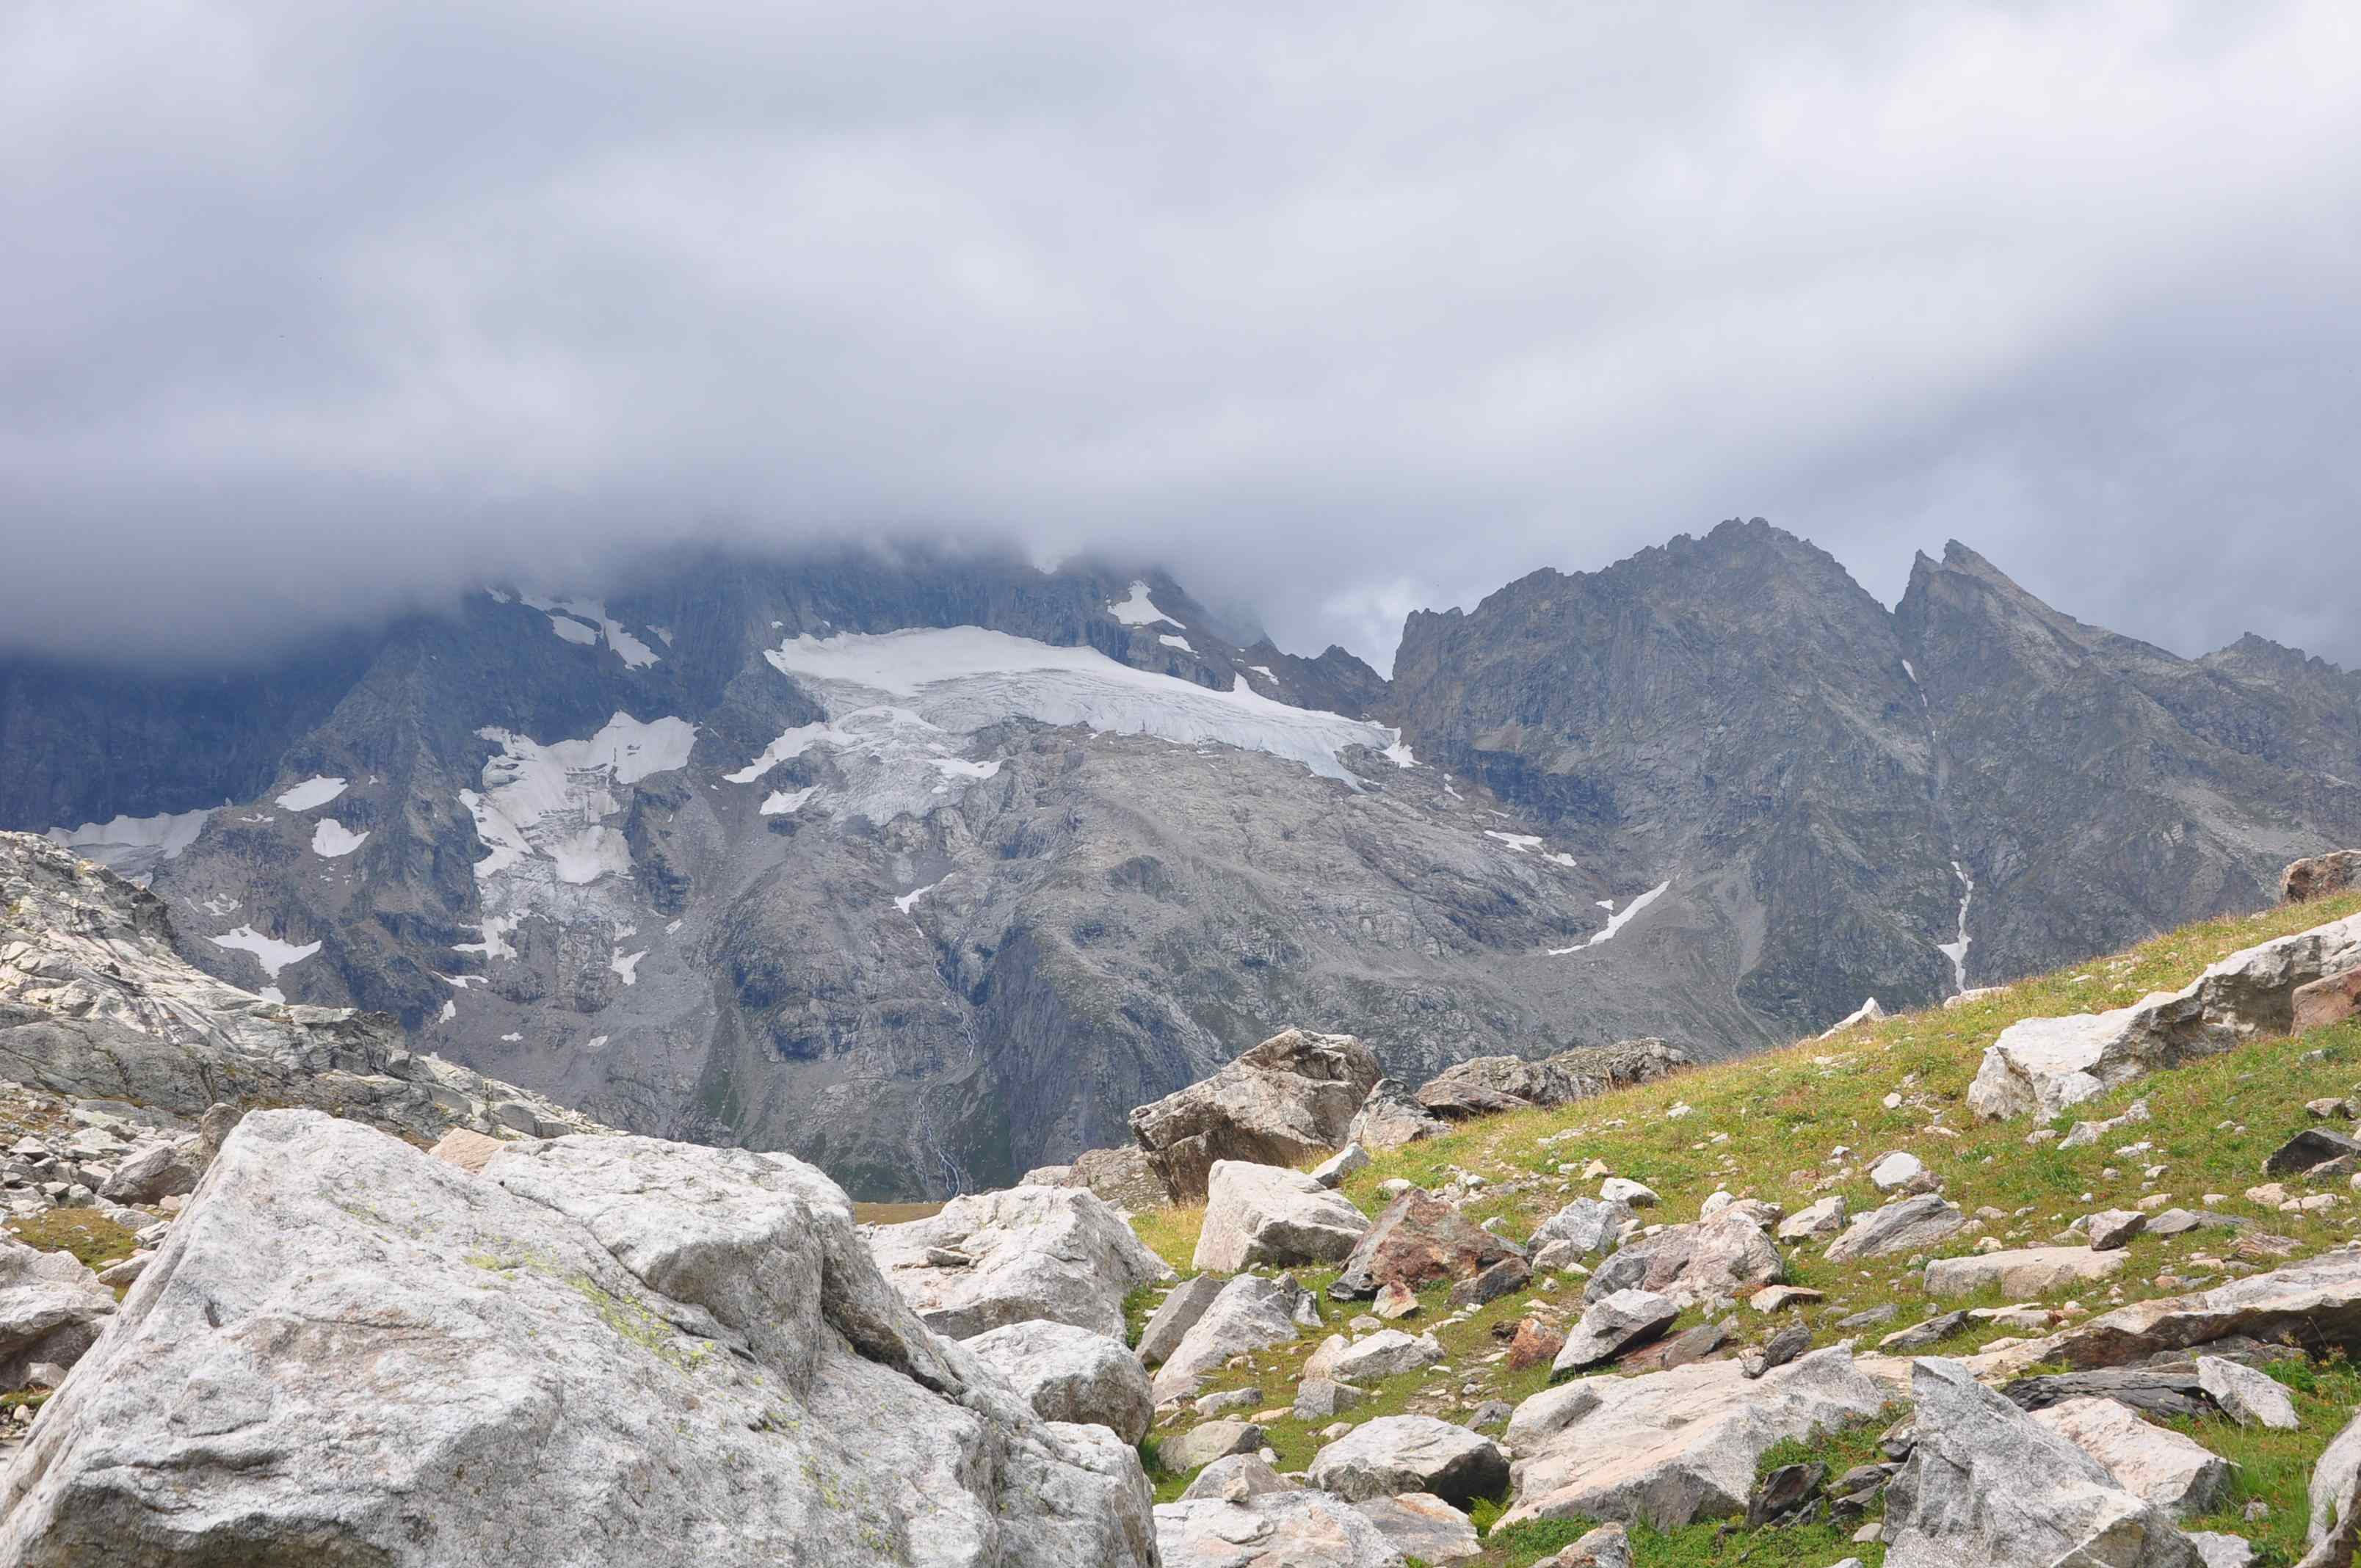
\includegraphics[width=\textwidth]{../pics/DSC_0222}			
\end{frame}

\begin{frame}
	\frametitle{Маршрут движения группы}
	\framesubtitle{День 9, 26 августа}
	\centering
	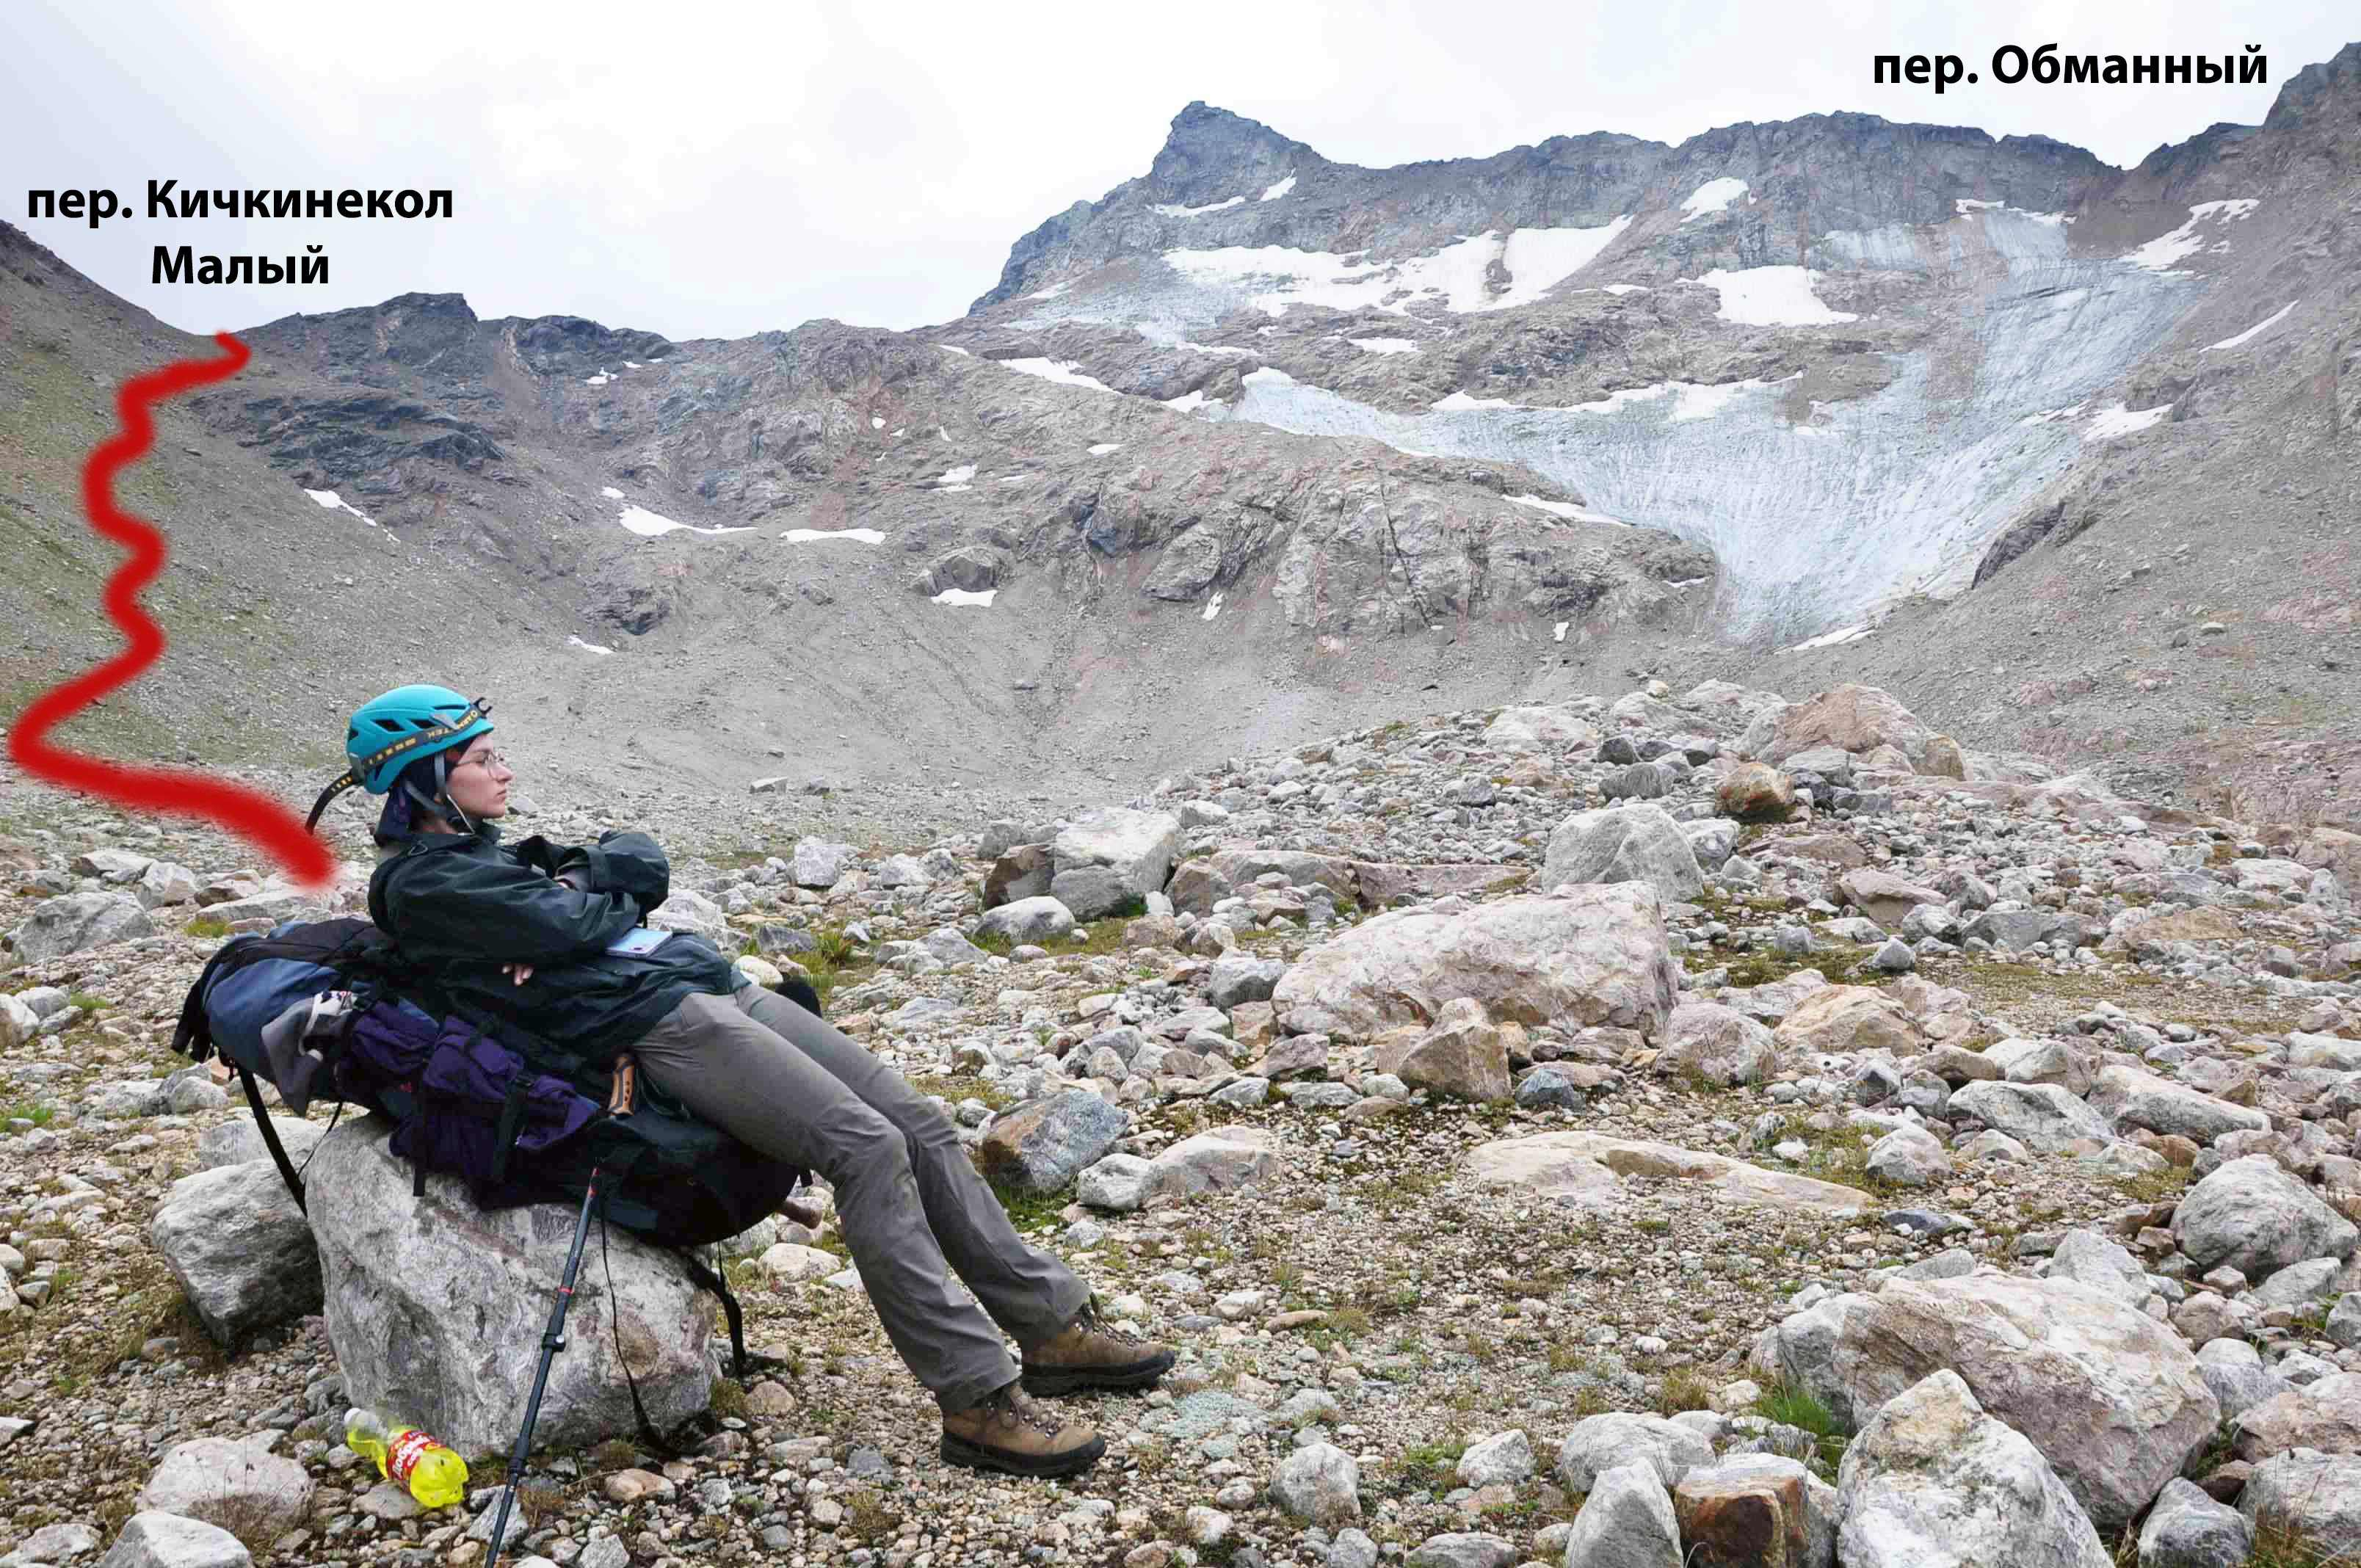
\includegraphics[width=\textwidth]{../pics/DSC_0226}			
\end{frame}


\begin{frame}
	\frametitle{Группа на пер. Кичкинекол Малый (1А)}
	\framesubtitle{День 9, 26 августа}
	{\tiny
		\begin{minipage}{\fourpicsize}
			\centering
			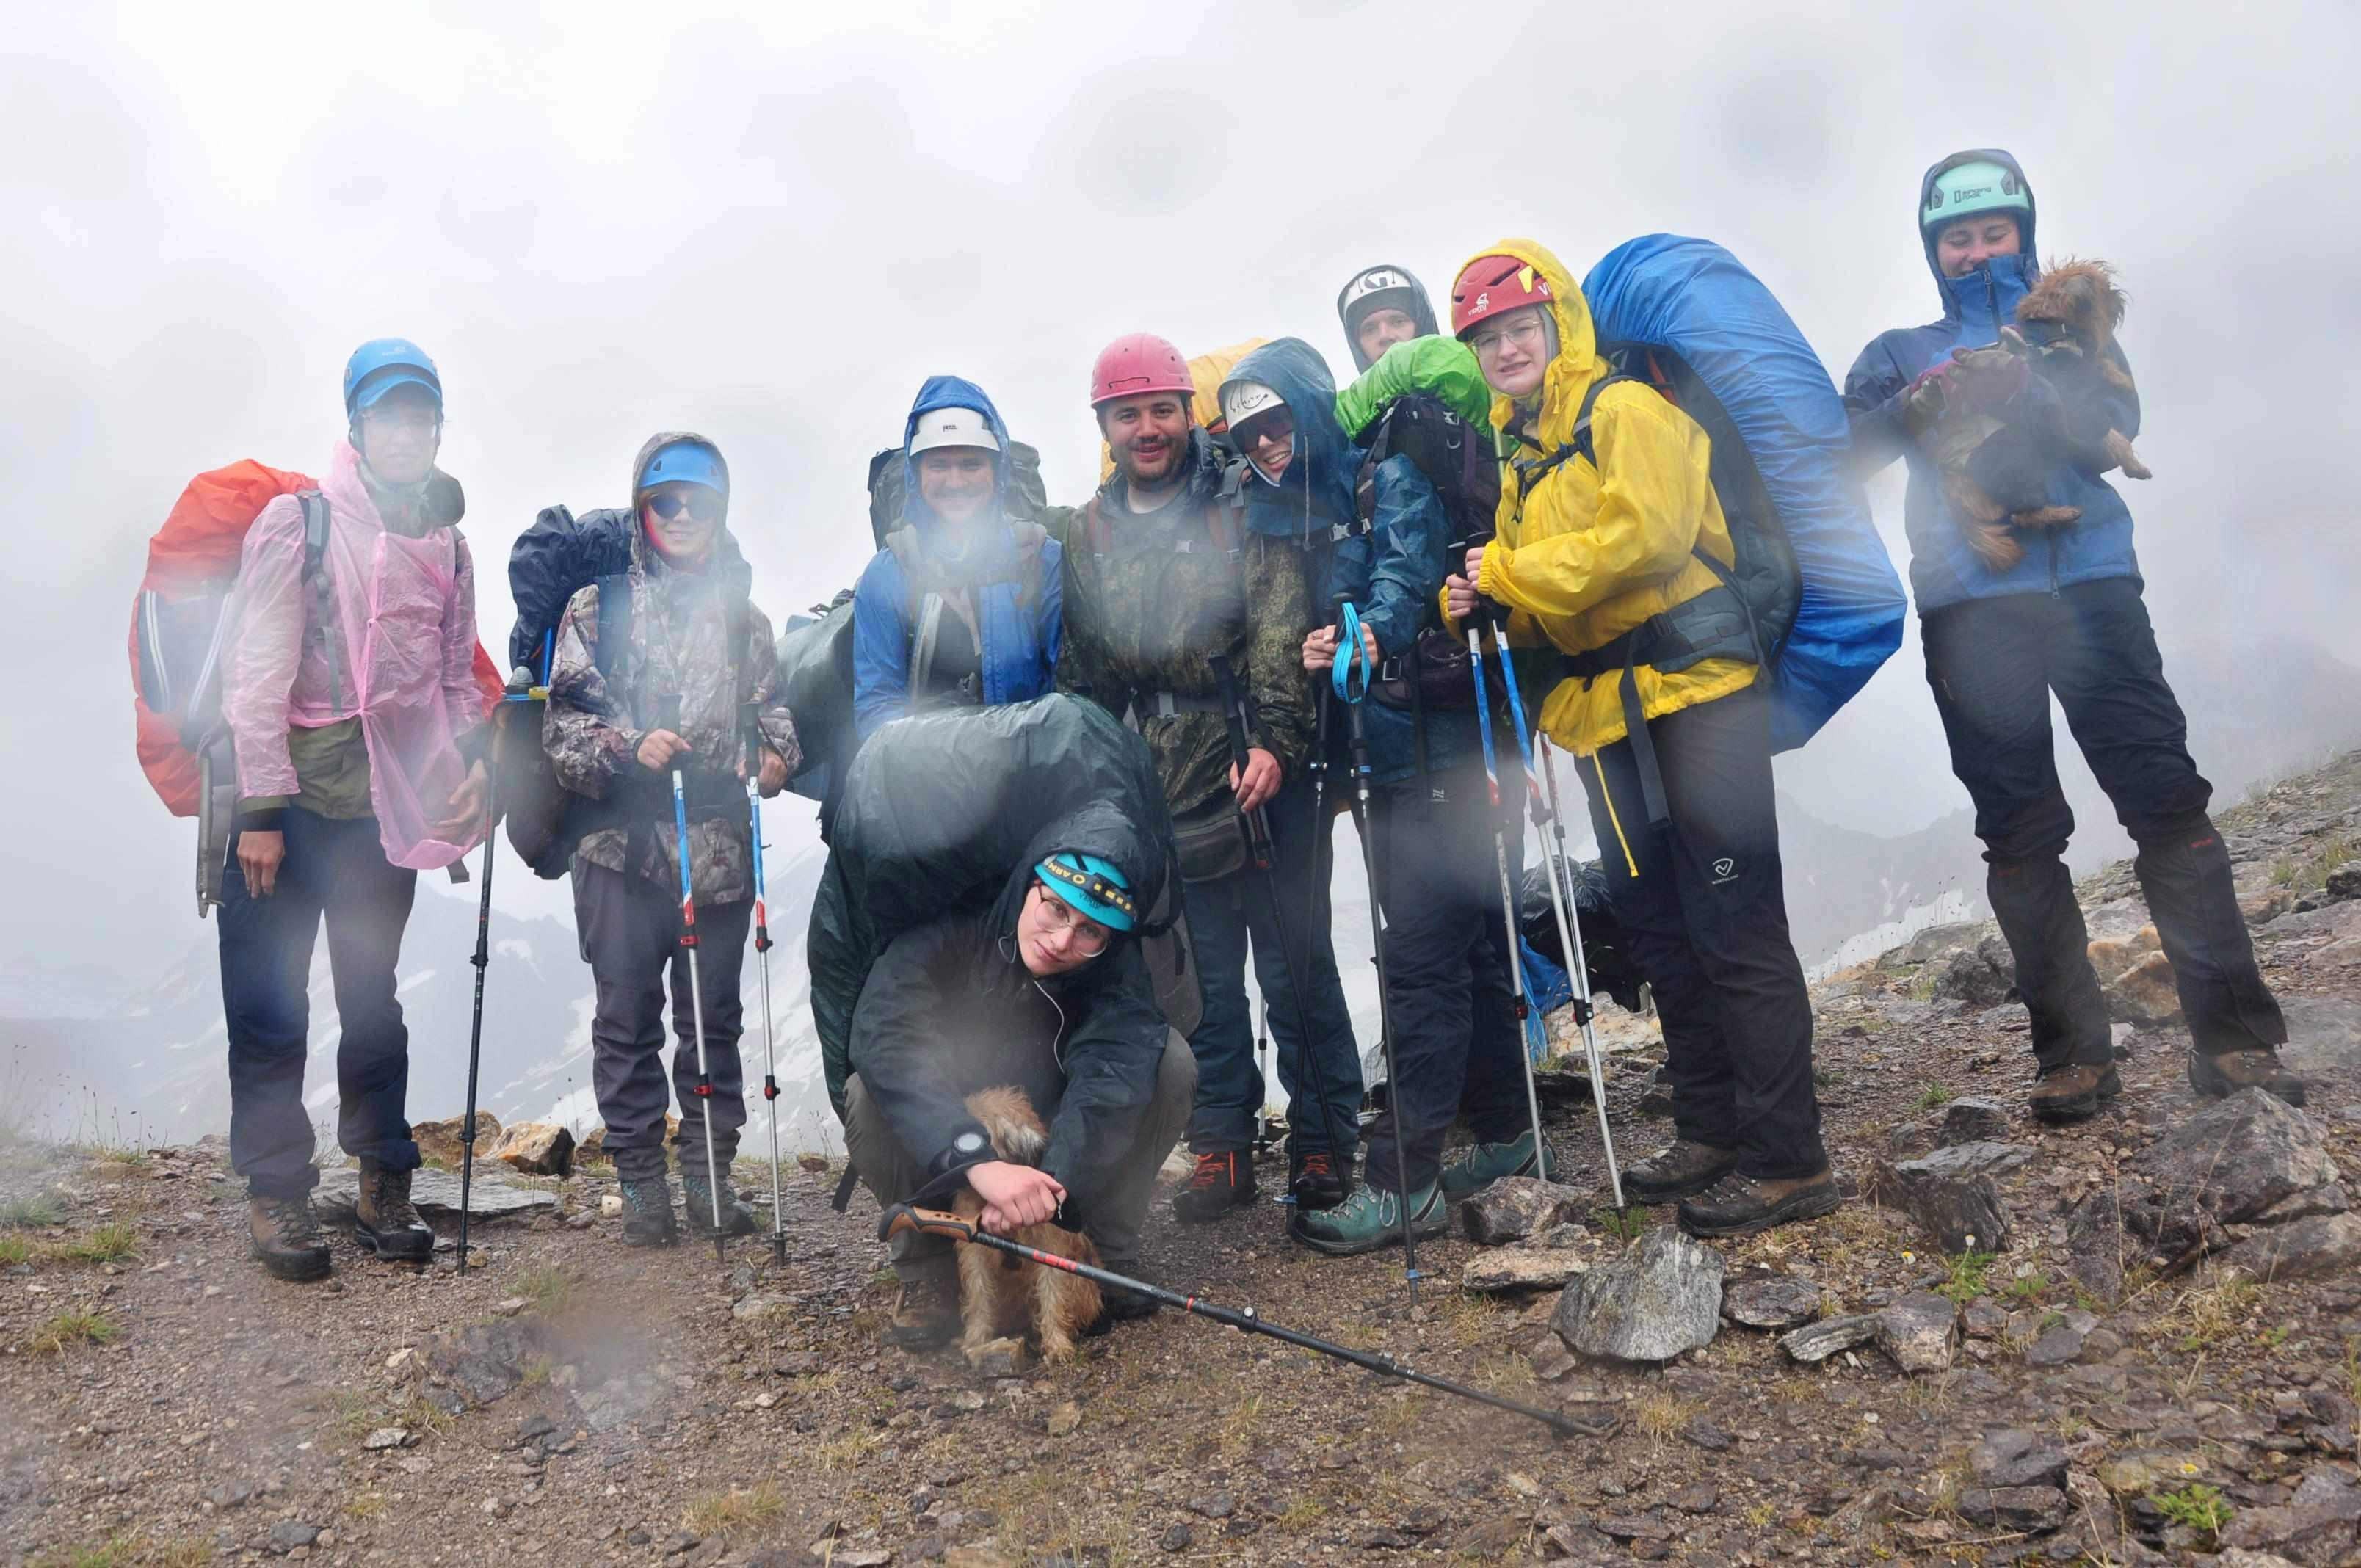
\includegraphics[width=\textwidth]{../pics/DSC_0239}			
			Вид в д.р. Чунгур-Джар
		\end{minipage}
		\hfill
		\begin{minipage}{\fourpicsize}
			\centering
			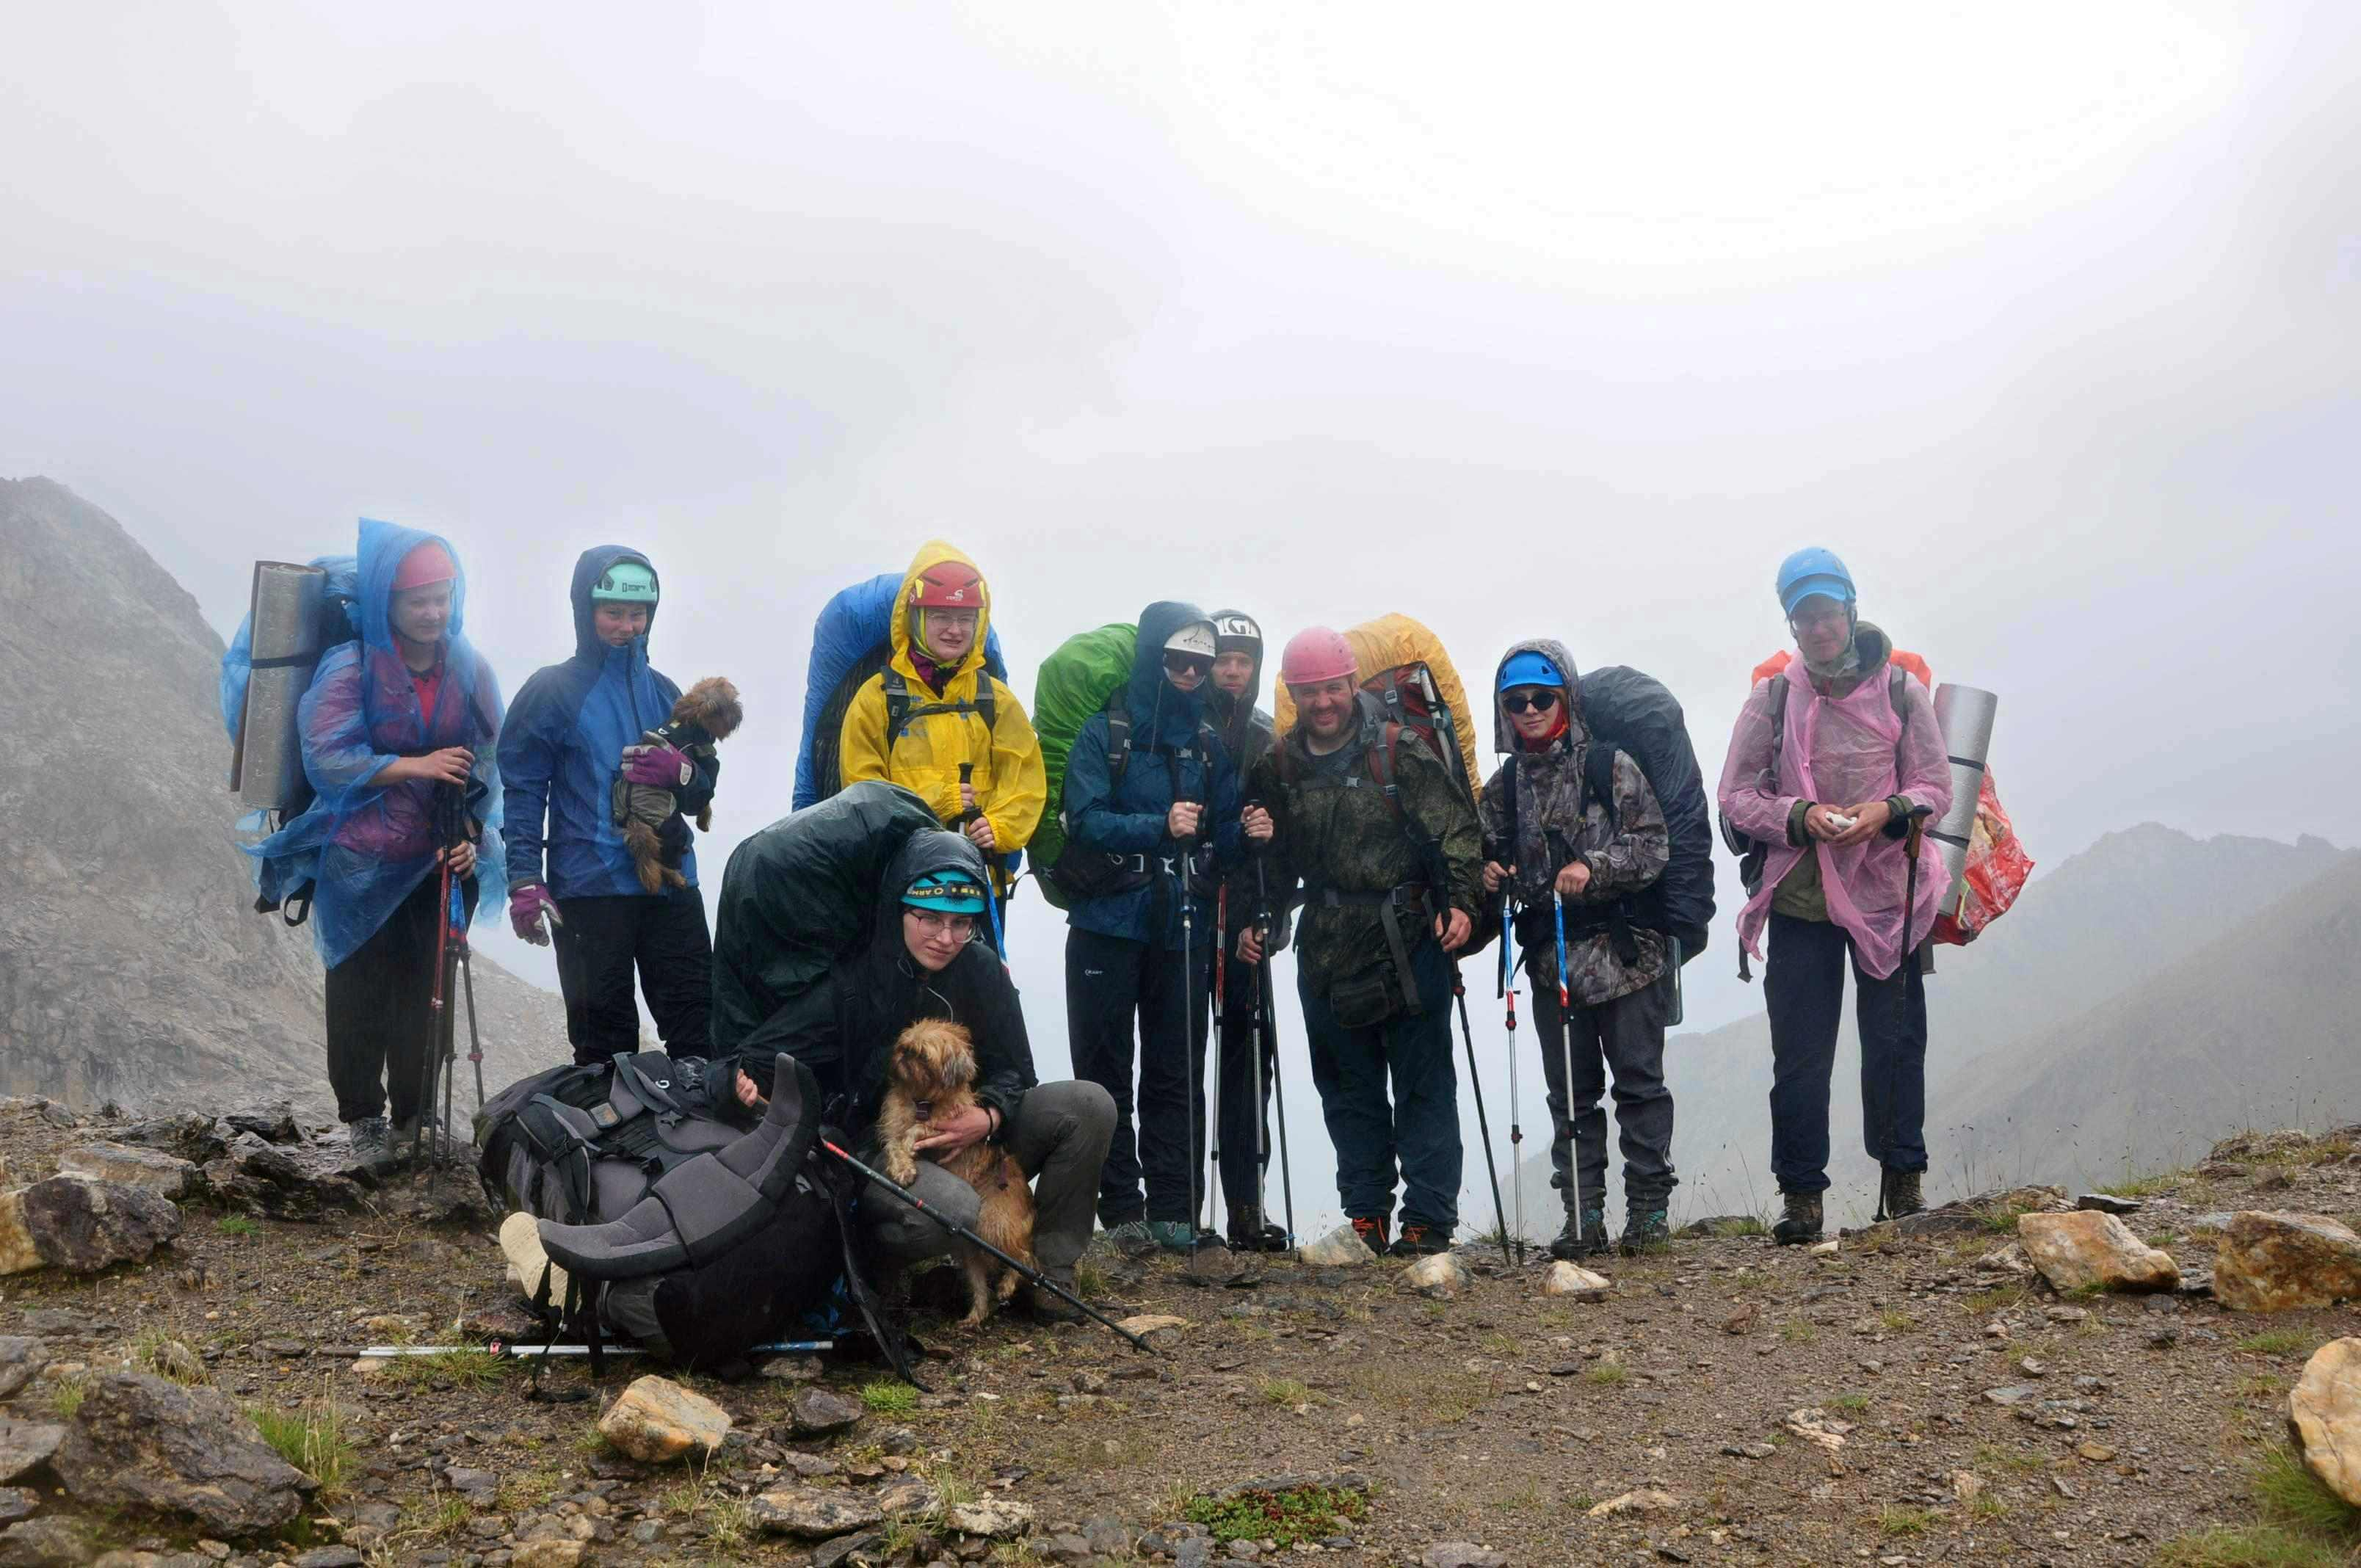
\includegraphics[width=\textwidth]{../pics/DSC_0242}			
			Вид в д.р. Таллычат
		\end{minipage}
		\vfill
	}
\end{frame}